\chapter{From Initial Data to Least Action}

These notes follow Leonard Susskind's second lecture on classical mechanics, as preserved in the course recording curated by LazyingArt LLC and Video2Book. The lecture opens as review, but it is not idle review. We begin with the question of initial conditions, use a deliberately false law to see what the order of a differential equation means, recover Newton's actual structure by contrast, review energy and momentum in that Newtonian setting, and then turn toward the deeper formulation in which one studies whole trajectories rather than local steps along them.

\section{First-Order and Second-Order Laws}

Susskind begins with one-dimensional motion and a false law of physics. The point is not to rescue Aristotle; it is to understand what a first-order equation would imply if nature had chosen one. The law is
\begin{equation}
F=m\dot x,
\end{equation}
or, if the force is known as a function of position,
\begin{equation}
F(x)=m\dot x.
\end{equation}
This law would say that in order to keep an object moving one must continuously exert a force on it. Remove the force, and the object comes immediately to rest. That is not our world. But mathematically the law is consistent, and that is enough for the comparison.

Suppose we know the position \(x\) at some instant. Then we know the force \(F(x)\). But the equation itself then tells us the velocity \(\dot x\). So for a first-order law of this kind, position already fixes the first time derivative. The natural question is whether it also fixes the higher derivatives. It does.

The force changes with time only because the particle moves through regions where the force differs. Therefore
\begin{equation}
\frac{dF}{dt}=\frac{dF}{dx}\,\dot x.
\end{equation}
Differentiating \(F(x)=m\dot x\) with respect to time gives
\begin{equation}
m\ddot x = \frac{dF}{dt}=\frac{dF}{dx}\,\dot x.
\end{equation}
So once the position is known, the velocity is known, and once the velocity is known, the acceleration is known. Differentiate once more:
\begin{align}
m\dddot x
&=
\frac{d}{dt}\!\left(\frac{dF}{dx}\,\dot x\right) \\
&=
\frac{d^2F}{dx^2}\,\dot x^{\,2}
+
\frac{dF}{dx}\,\ddot x.
\end{align}
The jerk is now determined as well. The pattern is obvious enough that Susskind is content to stop there: one can continue indefinitely, and each new time derivative is fixed by the previous ones and by derivatives of the force law. A first-order theory closes from position alone.

Now rerun the same question for Newton:
\begin{equation}
F(x)=m\ddot x.
\end{equation}
If we know the position, then we know the force, and therefore we know the acceleration. But the equation says nothing whatever about the velocity. The obstruction is immediate and decisive. A second-order equation does not propagate from position alone. To get started we must specify both
\begin{equation}
x(t_0),
\qquad
\dot x(t_0).
\end{equation}
Only then do we know enough to determine the acceleration, and from there the higher derivatives.

This is the first real lesson of the lecture: Newtonian mechanics is second order in time, and so its initial data are positions and velocities. For many particles the statement is the same in larger dimension: every coordinate and every corresponding velocity component must be supplied.

\subsection{Question \& Answer}

\paragraph{Question.} Why does Newton need both position and velocity while Aristotle's law did not?

\paragraph{Answer.} Because the issue is the order of the differential equation. In the first-order law \(F(x)=m\dot x\), knowing the position immediately gives the first derivative. In Newton's law \(F(x)=m\ddot x\), knowing the position gives only the second derivative. The first derivative remains independent, so velocity must be provided as part of the initial data.

\section{Conservative Forces and Energy Conservation}

Having reestablished the initial-data problem, Susskind turns to a quick review of energy conservation. He marks the level of the argument very clearly: the proof is elementary, but the principle is deeper than the proof. Energy conservation survives in electrodynamics, relativity, and quantum mechanics. Here we are only checking that Newton's equations reproduce it in the ordinary conservative case.

He first reminds us that not every force law conserves the mechanical sum of kinetic and potential energy. If we model friction crudely, the kinetic energy appears simply to disappear. Likewise, if some force kept pushing a particle around a circle in the same direction, the particle would come back to the same position with greater speed, so the kinetic energy would increase while the position, and hence any ordinary potential energy, returned to the same value. Such examples are a warning: the familiar energy law is not automatic.

The forces that occur in nature, at least in the Newtonian particle examples under discussion, are conservative. For a single particle they take the form
\begin{equation}
F_i=-\frac{\partial U}{\partial x_i},
\qquad
\vec F=-\nabla U.
\end{equation}
The minus sign is the content: force points in the direction of decreasing potential energy.

\begin{figure}[h]
\centering

\includegraphics[width=0.52\textwidth]{lecture_02_figure_02.png}
\caption{Energy definition and separate time-derivative terms. The top handwritten symbol is best read as \(T\), not \(E\); the transcript and the later cancellation make that normalization clear.}
\end{figure}

Now define the kinetic and total energies:
\begin{equation}
T=\frac12 mv^2=\frac12 m\sum_i v_i^2,
\qquad
E=T+U.
\end{equation}
The board in the lecture is worth preserving because it shows the order of the argument. First one writes down \(T\), then \(E=T+U\), then the separate derivatives of \(T\) and \(U\). Only afterward is the cancellation exposed.

The derivative of the kinetic energy is
\begin{align}
\frac{dT}{dt}
&=
\frac{d}{dt}\left(\frac12 m\sum_i v_i^2\right) \\
&=
\sum_i m v_i \frac{dv_i}{dt} \\
&=
\sum_i m v_i a_i.
\end{align}
The derivative of the potential energy follows from the chain rule:
\begin{align}
\frac{dU}{dt}
&=
\sum_i \frac{\partial U}{\partial x_i}\frac{dx_i}{dt} \\
&=
\sum_i \frac{\partial U}{\partial x_i}v_i.
\end{align}

\begin{figure}[h]
\centering

\includegraphics[width=0.78\textwidth]{lecture_02_figure_03.png}
\caption{Combined time derivative of the total energy and the force-minus-force cancellation.}
\end{figure}

Now add the two pieces:
\begin{align}
\frac{dE}{dt}
&=
\frac{dT}{dt}+\frac{dU}{dt} \\
&=
\sum_i \left(m a_i+\frac{\partial U}{\partial x_i}\right)v_i.
\end{align}
At this point the grouping on the board becomes transparent. We write \(m a_i=F_i\), while the conservative-force law says
\begin{equation}
\frac{\partial U}{\partial x_i}=-F_i.
\end{equation}
Therefore
\begin{equation}
\frac{dE}{dt}
=
\sum_i (F_i-F_i)v_i
=
0.
\end{equation}
That is the conservation of energy.

The lecture stresses not just the result but the rhythm of the proof. The two derivatives are built separately; only then are they collected into a bracket; and only then do we read the bracket as force minus force. This is review, but it is review with purpose. Already one feels that the conservation law is telling us something more organized than a mere equation of motion.

The same argument extends immediately to many-particle systems. The index \(i\) can stand not only for spatial directions but also for different particles. As long as the force on each coordinate is minus the derivative of the potential with respect to that coordinate, the total energy of the whole system is conserved.

\section{Force as the Time Derivative of Momentum}

Susskind now says, in effect, let us come to momentum. Again the mood is review, but the review is widening. Newton's law is rewritten in a slightly different form,
\begin{equation}
F_i=m\frac{dv_i}{dt}.
\end{equation}
Since the mass is constant, we may pull it inside the derivative:
\begin{equation}
F=\frac{d}{dt}(mv).
\end{equation}
And once we give \(mv\) a name,
\begin{equation}
\vec P = m\vec v,
\end{equation}
Newton's law becomes
\begin{equation}
\vec F=\frac{d\vec P}{dt}.
\end{equation}

\begin{figure}[h]
\centering

\includegraphics[width=0.52\textwidth]{lecture_02_figure_04.png}
\caption{Newton's law being rewritten in momentum form. This is a transition frame rather than a finished formula, but it preserves the live progression of the board.}
\end{figure}

\begin{figure}[h]
\centering

\includegraphics[width=0.52\textwidth]{lecture_02_figure_05.png}
\caption{Component and vector forms of force and momentum.}
\end{figure}

The board hierarchy in the lecture is worth reproducing in clean form:
\begin{align}
F_i &= m\frac{dv_i}{dt}, \\
F &= \frac{d}{dt}(mv), \\
\vec F &= \frac{d\vec P}{dt}.
\end{align}

Before going further, the lecture pauses for a sharp question: what assumptions about time are already buried in this Newtonian discussion? The answer is explicit. We are assuming a universal synchronized time, the same at every point in space. We are also assuming, for the moment, that the force law has no explicit time dependence. This is the most naive Newtonian picture, and the lecture wants that simplicity stated out loud before momentum conservation is derived within it.

Now take a closed system of particles. The force on each particle is the sum of forces due to all the others. For three particles,
\begin{align}
\vec F_1 &= \vec F_{12}+\vec F_{13}, \\
\vec F_2 &= \vec F_{21}+\vec F_{23}, \\
\vec F_3 &= \vec F_{31}+\vec F_{32}.
\end{align}
The notation is important: \(\vec F_{12}\) means the force on particle \(1\) due to particle \(2\). Newton's third law then says
\begin{equation}
\vec F_{12}=-\vec F_{21},
\qquad
\vec F_{13}=-\vec F_{31},
\qquad
\vec F_{32}=-\vec F_{23}.
\end{equation}
The last of these corrects a small slip in the transcripted cancellation line; the intended pair is clearly \(\vec F_{32}\) and \(\vec F_{23}\).

Since \(\dot{\vec P}_i=\vec F_i\), we have
\begin{align}
\frac{d\vec P_1}{dt} &= \vec F_{12}+\vec F_{13}, \\
\frac{d\vec P_2}{dt} &= \vec F_{21}+\vec F_{23}, \\
\frac{d\vec P_3}{dt} &= \vec F_{31}+\vec F_{32}.
\end{align}
Add them:
\begin{align}
\frac{d}{dt}\bigl(\vec P_1+\vec P_2+\vec P_3\bigr)
&=
\vec F_{12}+\vec F_{13}
+\vec F_{21}+\vec F_{23}
+\vec F_{31}+\vec F_{32} \\
&=0.
\end{align}
Hence
\begin{equation}
\frac{d\vec P_{\mathrm{tot}}}{dt}=0.
\end{equation}
So the total momentum of a closed system is conserved.

\begin{figure}[h]
\centering

\includegraphics[width=0.78\textwidth]{lecture_02_figure_06.png}
\caption{Pairwise force sketch for momentum conservation. The exact subscripts in the board drawing are not all legible, so the transcript controls the notation while the image preserves the layout and vector logic.}
\end{figure}

\begin{figure}[h]
\centering
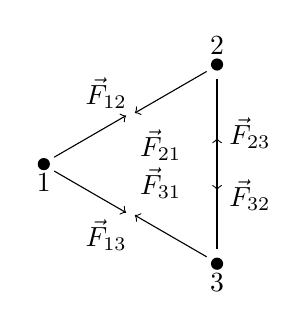
\begin{tikzpicture}[scale=1.1]
\fill (0,0) circle (2pt) node[below] {$1$};
\fill (2,1.15) circle (2pt) node[above] {$2$};
\fill (2,-1.15) circle (2pt) node[below] {$3$};

\draw[->] (0.12,0.08) -- (0.95,0.56);
\draw[->] (1.88,1.07) -- (1.05,0.59);
\node at (0.72,0.82) {$\vec F_{12}$};
\node at (1.35,0.22) {$\vec F_{21}$};

\draw[->] (0.12,-0.08) -- (0.95,-0.56);
\draw[->] (1.88,-1.07) -- (1.05,-0.59);
\node at (0.72,-0.82) {$\vec F_{13}$};
\node at (1.35,-0.22) {$\vec F_{31}$};

\draw[->] (2,0.98) -- (2,-0.30);
\draw[->] (2,-0.98) -- (2,0.30);
\node at (2.38,0.36) {$\vec F_{23}$};
\node at (2.38,-0.36) {$\vec F_{32}$};
\end{tikzpicture}
\caption{A cleaned pairwise-force diagram clarifying the cancellation of internal forces.}
\end{figure}

The lecture immediately widens the scope. Momentum conservation is far more general than this little Newtonian example suggests. It applies to light, to quantum mechanics, to relativity. The derivation we have given uses Newtonian assumptions, but the law itself is deeper.

\subsection{Question \& Answer}

\paragraph{Question.} Are action and reaction instantaneous, and which part of this argument is specifically Newtonian?

\paragraph{Answer.} In Newtonian mechanics, yes: forces are taken to act instantaneously, because time is assumed universal and signal propagation effectively infinite. That is the specifically Newtonian ingredient in the derivation. But the conservation of momentum itself survives when relativity removes instantaneous action at a distance. So the argument is Newtonian; the law is more general.

\section{A Mathematical Warm-Up: Stationary Points}

Only now does the lecture deliberately slow down and say: before we go on to the deep law of classical physics, we need a little mathematics. Not heavy mathematics, but just enough to put everyone back on the same playing field.

Take an ordinary function \(f(y)\) of one variable. If we look for a local minimum, the first condition is that the slope vanish:
\begin{equation}
\frac{df}{dy}=0.
\end{equation}
This condition is not sufficient to distinguish minima from maxima, and it also includes inflection points where the graph is momentarily flat. So the mathematically safer word is not minimum but stationary point. The function does not change to first order under a small change of the variable.

Susskind makes that point explicitly because the principle of least action is really the principle of stationary action. He says he will mostly keep the simpler phrase ``least action,'' but only after flagging the distinction.

For several variables the first-order condition simply splits into one equation per direction:
\begin{equation}
\frac{\partial f}{\partial x_i}=0
\qquad \text{for every } i.
\end{equation}
If the function is stationary, it must be stationary no matter which direction one moves away from the point.

The lecture then works a concrete two-variable example,
\begin{equation}
f(x,y)=x^2+y^2+3x+2y+xy+7.
\end{equation}
The stationary-point equations are
\begin{align}
\frac{\partial f}{\partial x} &= 2x+y+3=0, \\
\frac{\partial f}{\partial y} &= x+2y+2=0.
\end{align}
The constant \(7\) disappears, as it should: an overall vertical shift changes the height of the function but not the location of the stationary point. Solving the equations carefully gives
\begin{equation}
x=-\frac43,
\qquad
y=-\frac13.
\end{equation}
The lecture's spoken numbers are somewhat casual, but the equations themselves are stable, and the method is the point.

The transition is now ready. We know how to locate stationary points of ordinary functions. The next step is to study quantities that depend not on finitely many variables but on whole functions, whole curves, whole trajectories.

\subsection{Question \& Answer}

\paragraph{Question.} Is the principle really least action, or stationary action?

\paragraph{Answer.} Strictly speaking, stationary action. What must vanish is the first-order change in the quantity under a small deformation of the path. That condition includes minima, but it can also include maxima or other stationary cases. In the ordinary mechanical examples at hand, one often does have a minimum, and the lecture is content to speak that way, but the more accurate phrase is stationary action.

\section{Local Motion, Whole Paths, and Functionals}

At this point the lecture does something subtle. Before giving geometric examples, it restates the basic problem of mechanics itself. A mechanical system is described by generalized coordinates
\begin{equation}
q_1,\ q_2,\ \dots,\ q_n,
\end{equation}
which may be Cartesian coordinates, angles, orientations, latitude and longitude, or any other variables that locate the system in configuration space. The full motion is then the collection of functions
\begin{equation}
q_1(t),\ q_2(t),\ \dots,\ q_n(t).
\end{equation}
That collection is the generalized trajectory.

In the Newtonian formulation, to predict the future we must know the generalized coordinates and their time derivatives at one instant:
\begin{equation}
q_i(t_0),
\qquad
\dot q_i(t_0).
\end{equation}
Newton's equations are local equations along the trajectory. If we know where we are and how we are moving, the equations tell us the acceleration, and so they tell us how to proceed from one point of the trajectory to the next. One does not need knowledge of the whole curve in advance.

The principle of least action will formulate the same mechanics differently. Instead of the position and velocity at one time, we specify the positions at two times, the beginning and the end of the interval. That is a different but equally sufficient way to pose the problem. Susskind emphasizes this with the simple thought experiment of an object whose initial position is known and whose final position after one second is also known. The true trajectory is the one that connects those two endpoints in the allotted time.

Now the geometric examples can do their work. Consider first the shortest curve between two fixed points. Let \(y(x)\) describe the curve. For a small segment,
\begin{equation}
ds^2=dx^2+dy^2,
\end{equation}
so
\begin{equation}
ds=dx\sqrt{1+\left(\frac{dy}{dx}\right)^2}.
\end{equation}
Integrating from \(x_1\) to \(x_2\), the total length is
\begin{equation}
s_{12}[y]
=
\int_{x_1}^{x_2}
\sqrt{1+\left(\frac{dy}{dx}\right)^2}\,dx.
\end{equation}
This is not a function of a few variables. It is a rule that takes an entire function \(y(x)\) and returns a number. That is what the lecture now names: a functional.

The lecture insists on both a global and a local viewpoint. Globally, we minimize the total length of the whole curve. Locally, if we focus on a tiny segment between two nearby pinned points, the rule is simply: go straight ahead. The local differential-equation point of view and the global minimization point of view are different ways of expressing the same geometry.

There is also an instructive false shortcut. One might think that since the integrand contains \(1+(dy/dx)^2\), the shortest path should come from setting \(dy/dx=0\). But that would only produce a horizontal line, and a horizontal line will not generally pass through the fixed endpoints. The endpoint condition is part of the problem; one cannot minimize the integrand pointwise while ignoring the global constraint.

The optical example is even closer to what is coming in mechanics. Suppose the speed of light depends on height, \(c=c(y)\), as in a layered medium. Then
\begin{equation}
c(y)=\frac{ds}{dt},
\qquad
dt=\frac{ds}{c(y)}.
\end{equation}
Substituting the expression for \(ds\),
\begin{equation}
dt
=
\frac{\sqrt{1+\left(\frac{dy}{dx}\right)^2}}{c(y)}\,dx.
\end{equation}
Hence the total travel time is
\begin{equation}
t_{12}[y]
=
\int_{x_1}^{x_2}
\frac{\sqrt{1+\left(\frac{dy}{dx}\right)^2}}{c(y)}\,dx.
\end{equation}
The true light ray is the curve \(y(x)\) that makes this time stationary.

The lecture adds one more example in passing: a hanging chain of fixed length chooses the curve that minimizes its potential energy. The exact catenary formula is not derived here, but the point is the same. Physics repeatedly asks us to minimize quantities that depend on whole curves, not just on finitely many coordinates. That is the calculus of variations.

\section{The Action}

Only after this entire runway does Susskind finally say: now let me tell you what the action is. He presents it as something surprising and, even after decades, still surprising. The pedagogical rhythm matters. We are first invited to guess the wrong answer.

Take one particle moving in one dimension, with trajectory \(x(t)\). Since the action is to be built from kinetic and potential energy and integrated over time, the naive guess would be
\begin{equation}
\int_{t_0}^{t_1} (T+U)\,dt.
\end{equation}
That is the expected guess. But it is wrong.

The correct quantity is
\begin{equation}
A[x]
=
\int_{t_0}^{t_1}(T-U)\,dt
=
\int_{t_0}^{t_1}
\left(
\frac12 m\dot x^{\,2}-U(x)
\right)\,dt.
\end{equation}
This is the action. The integrand is called the Lagrangian:
\begin{equation}
L=T-U.
\end{equation}

At this point the lecture compares the action directly with the earlier functionals. In the least-distance problem the integrand depended on \(y(x)\) and on \(dy/dx\). In the least-time problem it depended on \(y(x)\), on \(dy/dx\), and on the local light speed \(c(y)\). Here, too, the integrand depends on the function and its first derivative: the position \(x(t)\) enters through the potential energy \(U(x)\), and the derivative \(\dot x\) enters through the kinetic energy.

This generalizes immediately. For a mechanical system with generalized coordinates \(q_i(t)\),
\begin{equation}
L(q,\dot q)=T-U,
\qquad
A[q]=\int_{t_0}^{t_1}L(q,\dot q)\,dt.
\end{equation}
In Newtonian particle mechanics the Lagrangian is the difference between kinetic and potential energy. In more general systems the Lagrangian may be a different function of \(q\) and \(\dot q\), but the action principle survives. That is why Susskind calls it the deepest law of classical physics.

The lecture also pauses over notation. Since \(s\) has already been used for path length, it is awkward to use \(s\) for action. The letter does not matter much, but the caution is sensible: the action is not to be confused with the distance functional we have just finished discussing.

The chapter should end where the lecture ends: at the threshold. The action has been revealed, but not yet varied. We have not derived the equations of motion from it. That task is deferred to the next lecture, where the analogy with optics will be completed and the least-action principle will be turned back into differential equations.

\subsection{Question \& Answer}

\paragraph{Question.} Why is the action built from kinetic minus potential energy rather than from the total energy?

\paragraph{Answer.} At the level of this lecture, the honest answer is that \(T-U\) is the combination that reproduces Newton's equations when the variational problem is worked out. Susskind explicitly postpones a deeper motivation and prefers first to examine the consequences. The minus sign is not ornamental. Once the potential is defined by \(F=-dU/dx\), the sign in the action determines the sign in the resulting equation of motion. The naive integral of \(T+U\) does not yield the Newtonian law in the form we want; the integral of \(T-U\) does.

\section{Summary}

The lecture begins with a question about initial conditions and ends with the action, but the argument unfolds in a very deliberate sequence. A false first-order law shows what it would mean for position alone to determine the whole motion. Newton's second-order law then shows why velocity must be supplied independently. Energy conservation is reviewed by building its ingredients separately and letting them cancel only at the end. Momentum conservation is derived from pairwise action and reaction, then immediately recognized as deeper than the Newtonian assumptions used in the derivation.

Only after that review does the lecture broaden its scope. We pass from stationary points of ordinary functions to functionals of whole curves, from local differential rules to global variational problems, and from fixed initial data to fixed endpoints. The payoff is the final formula
\begin{equation}
A[q]=\int_{t_0}^{t_1}L(q,\dot q)\,dt,
\qquad
L=T-U
\end{equation}
for Newtonian particle mechanics. The next step, and the next lecture's task, is to show how this global principle reproduces the local equations of motion.